\subsection{Chapter 2 - Comparing Model and Experiment}

\subsubsection{Overview}\label{chap:modelandexperiment}

In this chapter, we will learn about the process of doing science and lay the foundations for developing skills that will be of use throughout your scientific careers. In particular, we will start to learn how to test a model with an experiment, as well as learn to estimate whether a given result or model makes sense.

\begin{framed}
\textbf{Learning Objectives}\\
\begin{itemize}
\item Be able to estimate orders of magnitude.
\item Understand units.
\item Understand the process of building a model and performing an experiment.
\item Understand uncertainties in experiments.
\end{itemize}
\end{framed}

\begin{framed}
\textbf{Think About It}\\
Newton's Universal Theory of Gravity predicts that objects near the surface of the Earth will fall with an acceleration of $9.8{\rm m/s^2}$. Your friend reports that they have measured the acceleration of a falling ball and found that it was $9.0\pm 0.5 {\rm m/s^2}$. Does their result invalidate the prediction from Newton's Theory?\}

\begin{enumerate}
\item Yes, since the range $9.0\pm 0.5 {\rm m/s^2}$ does not include $9.8 {\rm m/s^2}$.
\item Not necessarily, as it depends on whether your friend correctly determined the uncertainty in their measurement.
\item Definitely not, since Newton's Universal Theory of Gravity has been confirmed by many experiments.
\end{enumerate}

\begin{framed}
\textbf{Answer}\\
\begin{enumerate}[resume]
\item
\end{enumerate}
\end{framed}
\end{framed}

\subsubsection{Orders of magnitude}

Although you should try to fight intuition when building a model to describe a particular phenomenon, you should not abandon critical thinking and should always ask if a prediction from your model makes sense. One of the most straightforward ways to estimate if a model makes sense is to ask whether it predicts the correct order of magnitude for a quantity. Usually, the order of magnitude for a quantity can be determined by making a very simple model, ideally one that you can work through in your head. When we say that a prediction gives the right ``order of magnitude'', we usually mean that the prediction is within a factor of ``a few'' (up to a factor of 10) of the correct answer. For example, if a measurement gives a value of 2000, then we would consider that a model prediction of 8000 gave the right order of magnitude (it differs from the correct answer by a factor of 4), whereas a prediction of 24000 would not (it differs by a factor of 12).

\begin{framed}
\textbf{Example 2.1}\\
How many ping pong balls can you fit into a school bus? Is it of order 10,000, or 100,000, or more?\}
Our strategy is to estimate the volumes of a school bus and of a ping pong ball, and then calculate how many times the volume of the ping pong ball fits into the volume of the school bus.

\begin{framed}
\textbf{Solution}\\
We can model a school bus as a box, say $20 {\rm m}\times 2 {\rm m}\times2 {\rm m}$, with a volume of $80 {\rm m^3}\sim 100 {\rm m^3}$. We can model a ping pong ball as a sphere with a diameter of $0.03 {\rm m} (3 {\rm cm}$). When stacking the ping pong balls, we can model them as little cubes with a side given by their diameter, so the volume of a ping pong ball, for stacking, is $\sim$ 0.00003 \{{\textbackslash}rm m\^3\}=3{\textbackslash}times 10\^\{-5\} ${\rm m^3}$. If we divide $100 {\rm m^3}$ by $3\times 10^{ -5} {\rm m^3}$, using scientific notation:
\begin{equation}
\frac{100 {\rm m^3}}{3\times 10^{-5} {\rm m^3}}=\frac{{1\times 10^{2}}}{{3\times 10^{-5}}}=\frac{1}{3}\times 10^7\sim 3\times 10^6
\end{equation}
Thus, we expect to be able to fit about three million ping pong balls in a school bus.

\begin{figure}[!htbp]
\centering
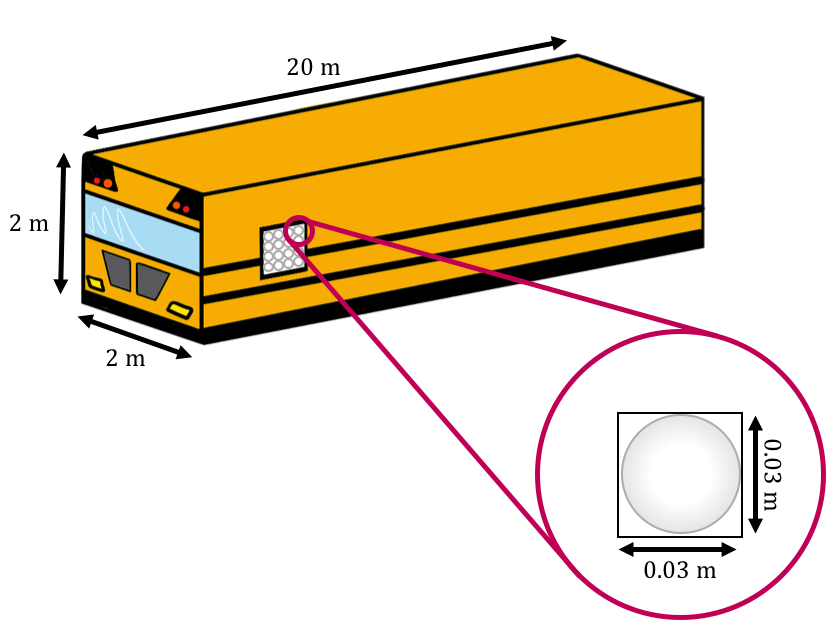
\includegraphics[width=0.55\linewidth]{files/schoolbusestimate-4f8ae92d39f3ff7dc9e6957709779c22.png}
\caption[]{A school bus and ping pong balls modelled as boxes.}
\label{fig:modelandexperiment:schoolbusestimate}
\end{figure}
\end{framed}
\end{framed}

\begin{framed}
\textbf{Checkpoint}\\
Fill in the following table, giving the order of magnitude (in meters) of the sizes of different physical objects. Feel free to look these up on the internet!

\begin{table}
\centering
\begin{tabular}{p{\dimexpr 0.500\linewidth-2\tabcolsep}p{\dimexpr 0.500\linewidth-2\tabcolsep}}
\toprule
\textbf{Object} & \textbf{Order of magnitude} \\
\hline
Proton &  \\
Nucleus of atom &  \\
Hydrogen atom &  \\
Virus &  \\
Human skin cell &  \\
Width of human hair &  \\
Human & $1 {\rm m}$ \\
Height of Mt. Everest &  \\
Radius of the Earth &  \\
Radius of the Sun &  \\
Radius of the Milky Way &  \\
\bottomrule
\end{tabular}
\end{table}

\begin{framed}
\textbf{Answer}\\
\begin{table}
\centering
\begin{tabular}{p{\dimexpr 0.500\linewidth-2\tabcolsep}p{\dimexpr 0.500\linewidth-2\tabcolsep}}
\toprule
\textbf{Object} & \textbf{Order of magnitude} \\
\hline
Proton & $10^{ -15} {\rm m}$ \\
Nucleus of atom & $10^{ -14} {\rm m}$ \\
Hydrogen atom & $10^{ -10} {\rm m}$ \\
Virus & $10^{ -7} {\rm m}$ \\
Human skin cell & $10^{ -5} {\rm m}$ \\
Width of human hair & $10^{ -4} {\rm m}$ \\
Human & $1 {\rm m}$ \\
Height of Mt. Everest & $10^{3} {\rm m}$ \\
Radius of the Earth & $10^{7} {\rm m}$ \\
Radius of the Sun & $10^{9} {\rm m}$ \\
Radius of the Milky Way & $10^{21} {\rm m}$ \\
\bottomrule
\end{tabular}
\end{table}
\end{framed}
\end{framed}

\subsubsection{Units and dimensions}

In 1999, the NASA Mars Climate Orbiter disintegrated in the Martian atmosphere because of a mixup in the units used to calculate the thrust needed to slow the probe and place it in orbit about Mars. A computer program provided by a private manufacturer used units of pounds seconds to calculate the change in momentum of the probe instead of the Newton seconds expected by NASA. As a result, the probe was slowed down too much and disintegrated in the Martian atmosphere. This example illustrates the need for us to \textbf{use and specify units} when we describe the properties of a physical quantity, and it also demonstrates the difference between a dimension and a unit.

``Dimensions'' can be thought of as types of measurements. For example, length and time are both dimensions. A unit is the standard that we choose to quantify a dimension. For example, meters and feet are both units for the dimension of length, whereas seconds and jiffys\footnote{A jiffy is a unit used in electronics and generally corresponds to either 1/50 or 1/60 seconds.} are units for the dimension of time.

When we compare two numbers, for example a prediction from a model and a measurement, it is important that both quantities have the same dimension {\textbackslash}textit\{and\} be expressed in the same units.

\begin{framed}
\textbf{Checkpoint}\\
The speed limit on a highway...

\begin{enumerate}
\item has the dimension of length over time and can be expressed in units of kilometers per hour.
\item has the dimension of length and can be expressed in units of kilometers per hour.
\item has the dimension of time over length and can be expressed in units of meters per second.
\item has the dimension of time and can be expressed in units of meters.
\end{enumerate}

\begin{framed}
\textbf{Answer}\\
\begin{enumerate}
\item
\end{enumerate}
\end{framed}
\end{framed}

\paragraph{Base dimensions and their SI units}

In order to facilitate communication of scientific information, the International System of units (SI for the french, Syst`eme International d'unit'es) was developed. This allows us to use a well-defined convention for which units to use when describing quantities. For example, the SI unit for the dimension of length is the meter and the SI unit for the dimension of time is the second.

In order to simplify the SI unit system, a fundamental (base) set of dimensions was chosen and the SI units were defined for those dimensions. Any other dimension can always be re-expressed in terms of the base dimensions shown in Table {\textbackslash}ref\{tab:modelandexperiment:SIunits\} and its units in terms of the corresponding combination of the base SI units.

\begin{table}
\centering
\caption[]{Base dimensions and their SI units with abbreviations.}
\label{tab:modelandexperiment:SIunits}
\begin{tabular}{p{\dimexpr 0.500\linewidth-2\tabcolsep}p{\dimexpr 0.500\linewidth-2\tabcolsep}}
\toprule
\textbf{Dimension} & \textbf{SI unit} \\
\hline
Length [L] & meter [m] \\
Time [T] & seconds[s] \\
Mass [M] & kilogram [kg] \\
Temperature [$\Theta$] & kelvin [K] \\
Electric current [I] & amp`ere [A] \\
Amount of substance [N] & mole [mol] \\
Luminous intensity [J] & candela [cd] \\
Dimensionless [1] & unitless [] \\
\bottomrule
\end{tabular}
\end{table}

From the base dimensions, one can obtain ``derived'' dimensions such as ``speed'' which is a measure of how fast an object is moving. The dimension of speed is $L/T$ (length over time) and the corresponding SI unit is m/s (meters per second)\footnote{Note that we can also write meters per second as m$\cdot$s\textsuperscript{-1}, but we often use a divide by sign if the power of the unit in the denominator is 1.}. Many of the derived dimension have corresponding derived SI units which can be expressed in terms of the base SI units. Table~\ref{tab:modelandexperiment:derivedSIunits} shows a few derived dimensions and their corresponding SI units and how those SI units are obtained from the base SI units.

\begin{table}
\centering
\caption[]{Example of derived dimensions and their SI units with abbreviations.}
\label{tab:modelandexperiment:derivedSIunits}
\begin{tabular}{p{\dimexpr 0.333\linewidth-2\tabcolsep}p{\dimexpr 0.333\linewidth-2\tabcolsep}p{\dimexpr 0.333\linewidth-2\tabcolsep}}
\toprule
\textbf{Dimension} & \textbf{SI unit} & \textbf{SI base units} \\
\hline
Speed [L/T] & meter per second [m/s] & [m/s] \\
Frequency [1/T] & hertz [Hz] & [1/s] \\
Force [M$\cdot$L$\cdot$T\textsuperscript{-2}] & newton [N] & [kg$\cdot$m$\cdot$s\textsuperscript{-2}] \\
Energy [M$\cdot$L$^2\cdot$T\textsuperscript{-2}] & joule [J] & [N$\cdot$m=kg$\cdot$m$^2\cdot$s\textsuperscript{-2}] \\
Power [M$\cdot$L$^2\cdot$T\textsuperscript{-3}] & watt [W] & [J/s=kg$\cdot$m$^2\cdot$s\textsuperscript{-3}] \\
Electric Charge [I$\cdot$ T] & coulomb [C] & [A$\cdot$ s] \\
Voltage [M$\cdot$L$^2\cdot$T$^{ -3}\cdot$I\textsuperscript{-1}] & volt [V] & [J/C=kg$\cdot$m$^2\cdot$s$^{ -3}\cdot$A\textsuperscript{-1}] \\
\bottomrule
\end{tabular}
\end{table}

By convention, we can indicate the dimension of a quantity, $X$, by writing it in square brackets, $[X]$. For example, $[X]=I$, would mean that the quantity $X$ has the dimension $I$, so it has the dimension of electric current. Similarly, we can indicate the SI units of $X$ with $SI[X]$. Referring to Table~\ref{tab:modelandexperiment:SIunits}, since $X$ has the dimension of current, $SI[X]=A$.

\paragraph{Dimensional analysis}

We call ``dimensional analysis'' the process of working out the dimensions of a quantity in terms of the base dimensions and a model prediction for that quantity. A few simple rules allow us to easily work out the dimensions of a derived quantity. Suppose that we have two quantities, $X$ and $Y$, both with dimensions. We then have the following rules to find the dimension of a quantity that depends on $X$ and $Y$:

\begin{enumerate}
\item Addition/Subtraction: You can only add or subtract two quantities if they have the same dimension: $[X+Y]=[X]=[Y]$
\item Multiplication: The dimension of the product, $[XY]$ , is the product of the dimensions: $[XY]=[X]\cdot[Y]$
\item Division: The dimension of the ratio, $[X/Y]$, is the ratio of the dimensions: $[X/Y]=[X]/[Y]$
\end{enumerate}

The next two examples show how to apply dimensional analysis to obtain the unit or dimension of a derived quantity.

\begin{framed}
\textbf{Example 2.2}\\
Acceleration has SI units of ${\rm ms^{ -2}}$ and force has the dimension of mass multiplied by acceleration. What are the dimensions and SI units of force, expressed in terms of the base dimensions and units?

\begin{framed}
\textbf{Solution}\\
We can start by expressing the dimension of acceleration, since we know from its SI units that it must have the dimension of length over time squared.
\begin{equation}
[{\rm acceleration}] = \frac{L}{T^2}
\end{equation}
Since force has the dimension of mass times acceleration, we have:
\begin{equation}
[{\rm force}] = [{\rm mass}]\cdot[{\rm acceleration}] = M \frac{L}{T^2}
\end{equation}
and the SI units of force are thus:
\begin{equation}
{\rm SI[force]} = {\rm kg}\cdot{\rm m/s^2}
\end{equation}
Force is such a common dimension that it, like many other derived dimensions, has its own derived SI unit, the Newton [N].
\end{framed}
\end{framed}

\begin{framed}
\textbf{Example 2.3}\\
Use Table~\ref{tab:modelandexperiment:derivedSIunits} to show that voltage has the same dimension as force multiplied by speed and divided by electric current.

\begin{framed}
\textbf{Solution}\\
According to Table~\ref{tab:modelandexperiment:derivedSIunits}, voltage has the dimension:
\begin{equation}
{\rm [voltage]=M\cdot L^2 \cdot T^{-3}\cdot I^{-1}}
\end{equation}
while force, speed and current have dimensions:
\begin{equation}
{\rm [force]}&={\rm M\cdot L\cdot T^{-2}} \\
{\rm [speed]}&={\rm L\cdot T^{-1}}\\
{\rm [current]}&={\rm I}
\end{equation}
The dimension of force multiplied by speed divided by electric charge
\begin{equation}
\left[\frac{\rm force\cdot speed}{\rm current}\right]&=\frac{\rm [force]\cdot [speed]}{\rm [current]}=\frac{\rm M\cdot L\cdot T^{-2} \cdot L\cdot T^{-1} }{\rm I}\\
&={\rm M\cdot L^2 \cdot T^{-3}\cdot I^{-1}}
\end{equation}
where, in the last line, we combined the powers of the same dimensions. By inspection, this is the same dimension as voltage.
\end{framed}
\end{framed}

When you build a model to predict the value of a physical quantity, you should always use dimensional analysis to ensure that the dimension of the quantity your model predicts is correct.

\begin{framed}
\textbf{Example 2.4}\\
Your model predicts that the speed, $v$, of an object of mass $m$, after having fallen a distance $h$ on the surface of a planet with mass $M$ and radius $R$ is given by:
\begin{equation}
v = \frac{mMh}{R}
\end{equation}
Is this a reasonable prediction?

\begin{framed}
\textbf{Solution}\\
First, we can see that the speed will be larger if $h$ is bigger, which makes sense, since we expect the speed to be greater if the object fell a greater distance. Similarly, we expect that the speed would be higher if the mass of the planet, $M$, is larger, as it would exert a larger gravitational force, as given by this model. We also expect that the object will have a greater speed if it has a larger mass, $m$, if the drag from the atmosphere on the planet is significant. Finally, if the radius of the planet $R$ is larger, we would expect the speed to be smaller, as the planet would be less dense and exert less gravitational force at its surface. However, if we verify the dimensions for the prediction of $v$, we find the model does not predict dimensions of speed:
\begin{equation}
[v] &= \frac{[m][M][h]}{[R]}\\
&=\frac{MML}{L}=M^2
\end{equation}
and our model predicts a speed with dimensions of mass squared. By performing simple dimensional analysis, we can easily confirm that our model is definitely wrong. You should always check the dimensions of any model prediction, to make sure it is correct.
\end{framed}
\end{framed}

\begin{framed}
\textbf{Olivia's Thoughts}\\
In this section, we were given three rules for combining dimensions. You'll notice that these rules are the same as the rules for algebra, except you're using dimensions instead of $x$'s and $y$'s. So, you can really just approach dimensional analysis problems as you would algebra problems.

There are some basic steps you can follow when you are trying to find the SI units for a value/variable in your equation. I'll go through Example~2.2 in a bit of a different way. Let's say that you have the equation $F=ma$ and this time, you know the dimensions of $F$ and $m$, and you want to find the dimensions of $a$:

\begin{enumerate}
\item Rewrite the values/variables in your equation in terms of their dimensions, leaving all other operations (multiplication, exponents, etc.) as is: $F=m\cdot a\rightarrow [F]=[m]\cdot[a]$
\item Rearrange for your unknown dimension: $[a]=\frac{[F]}{[m]}$
\item Substitute in your known dimensions: $[a]=\frac{[F]}{[m]} \rightarrow [a]=\frac{MLT^{ -2}}{M}=\frac{ML}{MT^2}$
\item Solve using the rules of algebra: $[a]=\frac{L}{T^2}$ (where we just cancelled out the $M$'s)
\item Replace the dimensions with their corresponding SI units: $[a]=\frac{L}{T^2}\rightarrow SI[a]=\frac{m}{s^2}$
\end{enumerate}
\end{framed}

\begin{framed}
\textbf{Checkpoint}\\
In Chloe's theory of falling objects from Section~\ref{chap:introduction}, the time, $t$, for an object to fall a distance, $x$, was given by $t=k\sqrt{x}$. What must the SI units of Chloe's constant, $k$, be?\}

\begin{enumerate}
\item ${\rm T.L^{\frac{1}{2}}}$
\item ${\rm T.L^{ -\frac{1}{2}}}$
\item ${\rm s.m^{\frac{1}{2}}}$
\item ${\rm s.m^{ -\frac{1}{2}}}$
\end{enumerate}

\begin{framed}
\textbf{Answer}\\
\begin{enumerate}[resume]
\item
\end{enumerate}
\end{framed}
\end{framed}

Dimensional analysis can also be used to determine formulas (usually to within an order of magnitude). One famous example of this is when a British physicist named G.I. Taylor was able to determine a formula that showed how the blast radius of an atomic bomb scaled with time. Using pictures of the first atomic bomb explosion, he was able to determine the amount of energy released in the explosion, which was classified information at the time.

\begin{framed}
\textbf{Example 2.5}\\
Find a formula that shows how the blast radius, $r$, scales with the time since the explosion, $t$, where the radius also depends on the energy released in the explosion, $E$, and the density of the medium into which the bomb explodes, $\rho$.

\begin{framed}
\textbf{Solution}\\
We want to find out how the blast radius scales with time, so we want an expression that relates $r$ to some combination of $E$, $\rho$, and $t$:
\begin{equation}
r \sim E^x\rho^y t^z
\end{equation}
where $x$, $y$, and $z$ are our unknown exponents, since we don't know yet how we will combine $E$, $\rho$, and $t$. However, we do know that when we combine these quantities, we have to get the correct dimension (length) for the radius:
\begin{equation}
[r]=[E]^x[\rho]^y[t]^z
\end{equation}
We know the dimensions for radius and time, and the dimension for $E$ can be found in Table {\textbackslash}ref\{tab:modelandexperiment:derivedSIunits\}. Density is mass divided by volume, so its dimension is $M/L^3$. Our equation then becomes:
\begin{equation}
L&=(ML^2T^{-2})^x(ML^{-3})^y(T)^z\\
L&=(M^xL^{2x}T^{-2x})(M^yL^{-3y})(T^z)\\
\end{equation}
We have three unknowns, so we need three equations. We can recognize that the left hand side (with dimension of length, $L$) is equivalent to $L^1\cdot M^0\cdot T^0$. We can then separate the above expression into three equations, one for each of $M$, $L$, and $T$:
\begin{equation}
M^0&=M^xM^y \rightarrow 0 = x+y\\
L^1&=L^{2x}L^{-3y} \rightarrow 1=2x-3y\\
T^0&=T^{-2x}T^{z} \rightarrow 0=z-2x
\end{equation}
Solving the sytem of equations, we find that $x=1/5$, $y= -1/5$, and $z=2/5$.
So, the combination of $E$, $\rho$, and $t$ that gives us the dimension of length is:
\begin{equation}
r\propto E^{1/5}\rho^{-1/5}t^{2/5}\\
\therefore r\propto t^{2/5}
\end{equation}
You can also write this equation as:
\begin{equation}
r\propto \sqrt[5]{\frac{Et^2}{\rho}}\\
\end{equation}
Thus, by measuring the blast radius at some time, and knowing the density of the air, you can estimate the energy that was released during the explosion.
\end{framed}
\end{framed}

\subsubsection{Making measurements}

Having introduced some tools for the modelling aspect of physics, we now address the other side of physics, namely performing experiments. Since the goal of developing theories and models is to describe the real world, we need to understand how to make meaningful measurements that test our theories and models.

Suppose that we wish to test Chloe's theory of falling objects from Section~\ref{chap:introduction}:
\begin{equation}
t=k\sqrt{x}
\end{equation}
which states that the time, $t$, for any object to fall a distance, $x$, near the surface of the Earth is given by the above relation. The theory assumes that Chloe's constant, $k$, is the same for any object falling any distance on the surface of the Earth.

One possible way to test Chloe's theory of falling objects is to measure $k$ for different drop heights to see if we always obtain the same value. Results of such an experiment are presented in Table {\textbackslash}ref\{tab:modelandexperiment:kmes\}, where the time, $t$, was measured for a bowling ball to fall distances of $x$ between $1 {\rm m}$ and $5 {\rm m}$. The table also shows the values computed for $\sqrt x$ and the corresponding value of $k=t/\sqrt x$:

\begin{table}
\centering
\caption[]{Measurements of the drop times, $t$, for a bowling ball to fall different distances, $x$. We have also computed $\sqrt x$ and the corresponding value of $k$.}
\label{tab:modelandexperiment:kmes}
\begin{tabular}{p{\dimexpr 0.250\linewidth-2\tabcolsep}p{\dimexpr 0.250\linewidth-2\tabcolsep}p{\dimexpr 0.250\linewidth-2\tabcolsep}p{\dimexpr 0.250\linewidth-2\tabcolsep}}
\toprule
\textbf{x} [m] & \textbf{t} [s] & \textbf{$\sqrt x$}  ${\rm \left[{m^{\frac{1}{2}}}\right]}$ & \textbf{k}  ${\rm \left[{s.m^{ -\frac{1}{2}}}\right]}$ \\
\hline
1.00 & 0.33 & 1.00 & 0.33 \\
2.00 & 0.74 & 1.41 & 0.52 \\
3.00 & 0.67 & 1.73 & 0.39 \\
4.00 & 1.07 & 2.00 & 0.54 \\
5.00 & 1.10 & 2.24 & 0.49 \\
\bottomrule
\end{tabular}
\end{table}

When looking at Table~\ref{tab:modelandexperiment:kmes}, it is clear that each drop height gave a different value of $k$, so at face value, we would claim that Chloe's theory is incorrect, as there does not seem to be a value of $k$ that applies to all situations. However, we would be incorrect in doing so unless we understood \textit{the precision of the measurements} that we made. Suppose that we \textbf{repeated} the measurement multiple times at a \textbf{fixed} drop height of $x=3 {\rm m}$, and obtained the values in Table~\ref{tab:modelandexperiment:kmes_3m}.

\begin{table}
\centering
\caption[]{Repeated measurements of the drop time, $t$, for a bowling ball to fall a distance $x=3 {\rm m}$. We have also computed $\sqrt x$ and the corresponding value of $k$.}
\label{tab:modelandexperiment:kmes_3m}
\begin{tabular}{p{\dimexpr 0.250\linewidth-2\tabcolsep}p{\dimexpr 0.250\linewidth-2\tabcolsep}p{\dimexpr 0.250\linewidth-2\tabcolsep}p{\dimexpr 0.250\linewidth-2\tabcolsep}}
\toprule
\textbf{x} [m] & \textbf{t} [s] & \textbf{$\sqrt x$}  ${\rm \left[{m^{\frac{1}{2}}}\right]}$ & \textbf{k}  ${\rm \left[{s.m^{ -\frac{1}{2}}}\right]}$ \\
\hline
3.00 & 1.01 & 1.73 & 0.58 \\
3.00 & 0.76 & 1.73 & 0.44 \\
3.00 & 0.64 & 1.73 & 0.37 \\
3.00 & 0.73 & 1.73 & 0.42 \\
3.00 & 0.66 & 1.73 & 0.38 \\
\bottomrule
\end{tabular}
\end{table}

This simple example highlights the critical aspect of making any measurement: it is impossible to make a measurement with infinite precision. The values in Table~\ref{tab:modelandexperiment:kmes_3m} show that if we repeat the exact same experiment, we are likely to measure different values for a single quantity. In this case, for a fixed drop height, $x=3 {\rm m}$, we obtained a spread in values of the drop time, $t$, between roughly $0.6 {\rm s}$ and $1.0 {\rm s}$. Does this mean that it is hopeless to do science, since we can never repeat measurements? Thankfully, no! It does however require that we deal with the inherent imprecision of measurements in a formal manner.

\paragraph{Measurement uncertainties}\label{sec:ModelAndExperiment:uncertainties}

The values in Table~\ref{tab:modelandexperiment:kmes_3m} show that for a fixed experimental setup (a drop height of $3 {\rm m}$), we are likely to measure a spread in the values of a quantity (the time to drop). We can quantify this ``uncertainty'' in the value of the measured time by quoting the measured value of $t$ by providing a ``central value'' and an ``uncertainty'':
\begin{equation}
t = 0.76 \pm 0.15 {\rm s}
\end{equation}
where $0.76 {\rm s}$ is called the ``central value'' and $0.15 {\rm s}$ the ``uncertainty'' or the ``error'. Note that we use the word error as a synonym for uncertainty, not ``mistake''. When we present a number with an uncertainty, we mean that we are ``pretty certain'' that the true value is in the range that we quote. In this case, the range that we quote is that $t$ is between $0.61 {\rm s}$ and $0.91 {\rm s}$ (given by $0.76 {\rm s} - 0.15 {\rm s}$ and $0.76 {\rm s} + 0.15 {\rm s}$). When we say that we are ``pretty sure'' that the value is within the quoted range, we usually mean that there is a 68\% chance of this being true and allow for the possibility that the true value is actually outside the range that we quoted. The value of 68\% comes from statistics and the normal distribution.

\begin{framed}
\textbf{Emma's Thoughts}\\
\textbf{``Precision'', ``Accuracy'' and ``Uncertainty'' - what's the difference?}

Have you ever started writing a lab report and wondered whether or not you should describe your measurement in terms of ``accuracy'' or ``precision''? What about describing the error in your experiment as a measure of ``accuracy'' or ``uncertainty''?

You're not alone! Precision, accuracy and uncertainty all relate to error, but have different meanings. To clarify these terms, I think it is useful to study them side-by-side.

\textbf{Precision} refers to how close your measurements are to each other when you repeat a measurement multiple times. If the values obtained are close to one another, your measurements are precise. For example, say you were measuring the rebound height of a basketball, dropped from a fixed height. After performing the measurement multiple times, you find that the measured rebound heights are very close in value to each other. You could then report that ``After repeating our measurement multiple times, the values that we obtained were very close together. Our measurements were precise!''. Of course, you have to specify what you mean by ``close'' (perhaps in terms of the divisions on the ruler that you used to measure rebound height).

\textbf{Accuracy} measures the agreement between a measured value and its true value. If the measured value is close to the true value, your measured value is accurate. For example, say that you developed a model for the distance covered by a rock thrown with a slingshot. If you find that the measured value is close to the predicted value, you would say that your model is accurate, ``Our model value was very close to the value that we measured - our model was accurate.'' Again, you have to specify what you mean by ``close'', usually in terms of the uncertainty on your measured value.

\textbf{Uncertainty} is an estimate of the amount that a measurement will differ from a true value. In science, we aim to lower the uncertainty in our measurements, so that we can test models and theories with more precision. Let's say that you are measuring the number of rotations of a spinning top during a certain period of time. Your measurements are close together, but have a fixed range of values. This would be an example where you could calculate the uncertainty in your measurements. It would be sensible to say ``After multiple measurements, we've found that our values are similar and our uncertainty captures the range of values that we measured.''
\end{framed}

\paragraph{Determining the central value and uncertainty}\label{sec:modelandexperiment:determiningu}

The tricky part when performing a measurement is to decide how to assign a central value and an uncertainty. For example, how did we come up with $t=0.76 \pm 0.15 {\rm s}$ from the values in Table~\ref{tab:modelandexperiment:kmes_3m}?

Determining the uncertainty and central value on a measurement is greatly simplified when one can repeat the same measurement multiple times, as we did in Table~\ref{tab:modelandexperiment:kmes_3m}. With repeatable measurements, a reasonable choice for the central value and uncertainty is to use the \textbf{mean} and \textbf{standard deviation} of the measurements, respectively.

If we have $N$ measurements of some quantity $t$, $\{t_1, t_2, t_3, \dots t_N\}$, then the mean, $\bar t$, and standard deviation, $\sigma_t$, are defined as:
\begin{equation}
\bar t &= \frac{1}{N}\sum_{i=1}^{i=N} t_i=\frac{t_1 +t_2 +t_3 +\dots+ t_N}{N} \\
\sigma_t^2 &=\frac{1}{N-1}\sum_{i=1}^{i=N}(t_i-\bar t)^2 = \frac{(t_1-\bar t)^2+(t_2-\bar t)^2+(t_3-\bar t)^2+\dots+(t_N-\bar t)^2}{N-1} \\
\sigma_t &=\sqrt{\sigma_t^2}
\end{equation}
The mean is just the arithmetic average of the values, and the standard deviation, $\sigma_t$, requires one to first calculate the mean, then the variance ($\sigma^2_t$, the square of the standard deviation). You should also note that for the variance, we divide by $N -1$ instead of $N$. The standard deviation and variance are quantities that come from statistics and are a good measure of how spread out the values of $t$ are about their mean, and are thus a good measure of the uncertainty.

\begin{framed}
\textbf{Example 2.6}\\
Calculate the mean and standard deviation of the values for $k$ from Table~\ref{tab:modelandexperiment:kmes_3m}.

\begin{framed}
\textbf{Solution}\\
In order to calculate the standard deviation, we first need to calculate the mean of the $N=5$ values of $k$: $\{0.58, 0.44, 0.37, 0.42, 0.38 \}$. The mean is given by:
\begin{equation}
\bar k = \frac{0.58 + 0.44 + 0.37 + 0.42 + 0.38}{5} = 0.44{\rm s.m^{-\frac{1}{2}}}
\end{equation}
We can now calculate the variance using the mean:
\begin{equation}
\sigma^2_k &= \frac{1}{4}[(0.58-0.44)^2+(0.44-0.44)^2\\
         &+(0.37-0.44)^2+(0.42-0.44)^2+(0.38-0.44)^2]=7.3e-3 {\rm s^2.m}
\end{equation}
and the standard deviation is then given by the square root of the variance:
\begin{equation}
\sigma_k=\sqrt{0.0073}=0.09{\rm s.m^{-\frac{1}{2}}}
\end{equation}
Using the mean and standard deviation, we would quote our value of $k$ as :
\begin{equation}
k=0.44 \pm 0.09{\rm s.m^{-\frac{1}{2}}}
\end{equation}
\end{framed}
\end{framed}

Any value that we measure will always have an uncertainty. In the case where we can easily repeat the measurement, we should do so to evaluate how reproducible it is, and the standard deviation of those values is usually a good first estimate of the uncertainty in a value\footnote{In practice, the standard deviation is an overly conservative estimate of the error and we would use the error on the mean, which is the standard deviation divided by the square root of the number of measurements.}. Sometimes, the measurements cannot easily be reproduced; in that case, it is still important to determine a reasonable uncertainty, but in this case, it usually has to be estimated.  Table~\ref{tab:modelandexperiment:uncertainties} shows a few common types of measurements and how to determine the uncertainties in those measurements.

\begin{table}
\centering
\caption[]{Different types of measurements and how to assign central values uncertainties.}
\label{tab:modelandexperiment:uncertainties}
\begin{tabular}{p{\dimexpr 0.500\linewidth-2\tabcolsep}p{\dimexpr 0.500\linewidth-2\tabcolsep}}
\toprule
\textbf{Type of measurement} & \textbf{How to determine central value and uncertainty} \\
\hline
Repeated measurements & Mean and standard deviation \\
Single measurement with a graduated scale (e.g. ruler, digital scale, analogue meter) & Closest value and half of the smallest division \\
Counted quantity & Counted value and square root of the value \\
\bottomrule
\end{tabular}
\end{table}

\begin{figure}[!htbp]
\centering
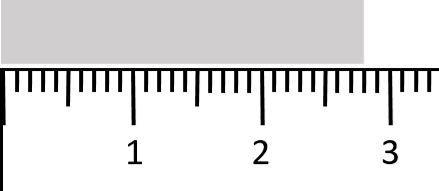
\includegraphics[width=0.4\linewidth]{files/ruler-363cbcff3850a55b9c486b9bbf87b570.png}
\caption[]{The length of the grey rectangle would be quoted as $L=2.8\pm0.05 {\rm cm}$ using the rule of ``half the smallest division''.}
\label{fig:modelandexperiment:ruler}
\end{figure}

For example, we would quote the length of the grey object in Figure~\ref{fig:modelandexperiment:ruler} to be $L=2.8\pm0.05 {\rm cm}$ based on the rules in Table~\ref{tab:modelandexperiment:uncertainties}, since $2.8 {\rm cm}$ is the closest value on the ruler that matches the length of the object and $0.5 {\rm mm}$ is half of the smallest division on the ruler. Using half of the smallest division of the ruler means that our uncertainty range covers one full division. Note that it is usually better to reproduce a measurement to evaluate the uncertainty instead of using half of the smallest division, although half of the smallest division should be the lower limit on the uncertainty. That is, by repeating the measurements and obtaining the standard deviation, you should see if the uncertainty is \textit{larger} than half of the of the smallest division, not smaller.

The \textbf{relative uncertainty} in a measured value is given by dividing the uncertainty by the central value, and expressing the result as a percent. For example, the relative uncertainty in $t=0.76\pm 0.15 {\rm s}$ is given by $0.15/0.76=20\%$. The relative uncertainty gives an idea of how precisely a value was determined. Typically, a value above 10\% means that it was not a very precise measurement, and we would generally consider a value smaller than 1\% to correspond to quite a precise measurement.

\subparagraph{Random and systematic sources of error/uncertainty}

It is important to note that there are two possible sources of uncertainty in a measurement. The first is called ``statistical'' or ``random'' and occurs because it is impossible to exactly reproduce a measurement. For example, every time you lay down a ruler to measure something, you might shift it slightly one way or the other which will affect your measurement. The important property of random sources of uncertainty is that if you reproduce the measurement many times, these will tend to cancel out and the mean can usually be determined to high precision with enough measurements.

The other source of uncertainty is called ``systematic''. Systematic uncertainties are much more difficult to detect and to estimate. One example would be trying to measure something with a scale that was not properly tarred (where the 0 weight was not set). You may end up with very small random errors when measuring the weights of object (very repeatable measurements), but you would have a hard time noticing that all of your weights were offset by a certain amount unless you had access to a second scale. Some common examples of systematic uncertainties are: incorrectly calibrated equipment, parallax error when measuring distance, reaction times when measuring time, effects of temperature on materials, etc.

As a reminder, we want to emphasize the difference between ``error'' and ``mistake'' in the context of making measurements. ``Uncertainty'' or ``error'' in a measurement comes from the fact that it is impossible to measure anything to infinite accuracy. A ``mistake'' also affects a measurement, but is preventable. If a ``mistake'' occurs in physics, the experiment is generally re-done and the previous data are discarded. The term ``human error'' should never be used in a lab report as it implies that a mistake was made. Instead, if you think that you measured time imprecisely, for example, refer to ``human reaction time'', not ``human error''.

Table~\ref{tab:modelandexperiment:humanerror} shows examples of sources of error that students often call ``human error'' but that should, instead, be described more precisely.

\begin{table}
\centering
\caption[]{Don't use the term ``human error'', instead, use these.}
\label{tab:modelandexperiment:humanerror}
\begin{tabular}{p{\dimexpr 0.500\linewidth-2\tabcolsep}p{\dimexpr 0.500\linewidth-2\tabcolsep}}
\toprule
\textbf{Situation} & \textbf{Source of Error} \\
\hline
While taking measurements, your line of sight was not completely parallel to the measuring device. & This is parallax error - a type of systematic error. \\
You incorrectly performed calculations. & Mistake! Redo the calculations. \\
A draft of wind in the lab slightly altered the direction of your ball rolling down an incline. & This is an environmental effect/error - it could be random or systematic, depending on whether it always had the same effect. \\
Your hand slipped while holding the ruler - the object was measured to be twice its original size! & Mistake! Redo this experiment and discard the data. \\
When timing an experiment, you don't hit the ``STOP'' button exactly when the experiment stops. & Reaction time error - usually a systematic error (time is usually measured longer than it is). \\
\bottomrule
\end{tabular}
\end{table}

\subparagraph{Propagating uncertainties}

Going back to the data in Table~\ref{tab:modelandexperiment:kmes_3m}, we found that for a known drop height of $x=3 {\rm m}$, we measured different values of the drop time, which we found to be $t=0.76 \pm 0.15 {\rm s}$ (using the mean and standard deviation). We also calculated a value of $k$ corresponding to each value of $t$, and found $k=0.44 \pm 0.09{\rm s.m^{ -\frac{1}{2}}}$ (Example~2.6).

Suppose that we did not have access to the individual values of $t$, but only to the value of $t=0.76 \pm 0.15 {\rm s}$ with uncertainty. How do we calculate a value for $k$ with uncertainty? In order to answer this question, we need to know how to ``propagate'' the uncertainties in a measured value to the uncertainty in a value derived the measured value. We briefly present different methods for propagating uncertainties, before advocating for the use of computers to do the calculations for you.

\begin{enumerate}
\item \textbf{Estimate using relative uncertainties} The relative uncertainty in a measurement gives us an idea of how precisely a value was determined. Any quantity that depends on that measurement should have a precision that is similar; that is, we expect the relative uncertainty in $k$ to be similar to that in $t$. For $t$, we saw that the relative uncertainty was approximately 20\%. If we take the central value of $k$ to be the central value of $t$ divided by $\sqrt x$, we find:
\end{enumerate}
\begin{equation}
k=\frac{(0.76 {\rm s})}{\sqrt{(3 {\rm m})}}=0.44{\rm s.m^{-\frac{1}{2}}}
\end{equation}
Since we expect the relative uncertainty in $k$ to be approximately 20\%, then the absolute uncertainty is given by:
\begin{equation}
\sigma_k = (0.2) k=0.09 {\rm s.m^{-\frac{1}{2}}}
\end{equation}
which is close to the value obtained by averaging the five values of $k$ in Table~\ref{tab:modelandexperiment:kmes_3m}.

\begin{enumerate}[resume]
\item \textbf{The Min-Max method} A pedagogical way to determine $k$ and its uncertainty is to use the ``Min-Max method''. Since $k=t/\sqrt x$, $k$ will be the biggest when $t$ is the biggest, and the smallest when $t$ is the smallest. We can thus determine ``minimum'' and ``maximum'' values of $k$ corresponding to the minimum value of $t$, $t^{min}=0.61 {\rm s}$ and the maximum value of $t$, $t^{max}=0.91 {\rm s}$:
\end{enumerate}
\begin{equation}
k^{min} &= \frac{t^{min}}{\sqrt x}=\frac{0.61\,s}{\sqrt{(3\,m)}} = 0.35 {\rm s.m^{-\frac{1}{2}}}\\
k^{max} &= \frac{t^{max}}{\sqrt x}=\frac{0.91\,s}{\sqrt{(3\,m)}} = 0.53{\rm s.m^{-\frac{1}{2}}}\\
\end{equation}
This gives us the range of values of $k$ that correspond to the range of values of $t$. We can choose the middle of the range as the central value of $k$ and half of the range as the uncertainty:
\begin{equation}
\bar k &= \frac{1}{2}(k^{min}+k^{max})= 0.44 {\rm s.m^{-\frac{1}{2}}}\\
\sigma_k &= \frac{1}{2}(k^{max}-k^{min})= 0.09 {\rm s.m^{-\frac{1}{2}}}\\
\therefore k&= 0.44 \pm 0.09 {\rm s.m^{-\frac{1}{2}}}
\end{equation}
which, in this case, gives the same value as that obtained by averaging the individual values of $k$. While the Min-Max method is useful for illustrating the concept of propagating uncertainties, we usually do not use it in practice as it tends to overestimate the uncertainty.

\begin{enumerate}[resume]
\item \textbf{The derivative method} In the example above, we assumed that the value of $x$ was known precisely (and we chose 3,m), which of course is not realistic. Let us suppose that we have measured $x$ to within $1 {\rm cm}$ so that $x=3.00 \pm 0.01 {\rm m}$. The task is now to calculate $k=\frac{t}{\sqrt{x}}$ when both $x$ and $t$ have uncertainties.
\end{enumerate}

The derivative method lets us propagate the uncertainty in a general way, so long as the relative uncertainties on all quantities are ``small'' (less than 10-20\%). If we have a function, $F(x,y)$ that depends on multiple variables with uncertainties (e.g. $x\pm\sigma_x$, $y\pm\sigma_y$), then the central value and uncertainty in $F(x,y)$ are given by:
\begin{equation}
\bar F &= F(\bar x, \bar y) \nonumber \\
\sigma_F &= \sqrt{\left(\frac{dF}{dx}\sigma_x \right)^2 + \left(\frac{dF}{dy}\sigma_y \right)^2 }
\end{equation}
That is, the central value of the function $F$ is found by evaluating the function at the central values of $x$ and $y$. The uncertainty in $F$, $\sigma_F$, is found by taking the quadrature sum of the partial derivatives of $F$ evaluated at the central values of $x$ and $y$ multiplied by the uncertainties in the corresponding variables that $F$ depends on. The uncertainty will contain one term in the sum per variable that $F$ depends on.

In \href{\#app:python}{Appendix D}, we will show you how to calculate this easily with a computer, so do not worry about getting comfortable with partial derivatives (yet!). Note that the partial derivative, $\frac{dF}{dx}$, is simply the derivative of $F(x,y)$ relative to $x$ evaluated as if $y$ were a constant. Also, when we say ``add in quadrature'', we mean square the quantities, add them, and then take the square root (same as you would do to calculate the hypotenuse of a right-angle triangle).

\begin{framed}
\textbf{Example 2.7}\\
Use the derivative method to evaluate $k=\frac{t}{\sqrt{x}}$ for $x=3.00 \pm 0.01 {\rm m}$ and $t=0.76\pm0.15 {\rm s}$.

\begin{framed}
\textbf{Solution}\\
Here, $k=k(x,t)$ is a function of both $x$ and $t$. The central value is easily found using the central values for $x$ and $t$:
\begin{equation}
\bar k = \frac{t}{\sqrt{x}} = \frac{(0.76 {\rm s})}{\sqrt{(3 {\rm m})}}= 0.44 {\rm s.m^{-\frac{1}{2}}}
\end{equation}
Next, we need to determine and evaluate the partial derivative of $k$ with respect to $t$ and $x$:
\begin{equation}
\frac{dk}{dt}&=\frac{1}{\sqrt{x}}\frac{d}{dt}t=\frac{1}{\sqrt{x}}=\frac{1}{\sqrt{(3 {\rm m})}}=0.58 {\rm m^{-\frac{1}{2}}}\\
\frac{dk}{dx}&=t\frac{d}{dx}x^{-\frac{1}{2}}=-\frac{1}{2}tx^{-\frac{3}{2}}= -\frac{1}{2}(0.76 {\rm s})(3.00 {\rm m})^{-\frac{3}{2}}=-0.073 {\rm s.m^{-\frac{3}{2}}}
\end{equation}
And finally, we plug this into the quadrature sum to get the uncertainty in $k$:{\textbackslash}
\begin{equation}
\sigma_k&=\sqrt{\left(\frac{dk}{dx}\sigma_x \right)^2 + \left(\frac{dk}{dt}\sigma_t \right)^2 }\\
&= \sqrt{\left((0.073 {\rm s.m^{-\frac{3}{2}}}) (0.01 {\rm m}) \right)^2 + \left((0.58 {\rm m^{-\frac{1}{2}}})(0.15 {\rm s}) \right)^2 } \\
&=0.09 {\rm s.m^{-\frac{1}{2}}}
\end{equation}
So we find that:
\begin{equation}
k&= 0.44 \pm 0.09 {\rm s.m^{-\frac{1}{2}}}
\end{equation}
which is consistent with what we found with the other two methods.

\textbf{Discussion:} We should ask ourselves if the value we found is reasonable, since we also included an uncertainty in $x$ and would expect a bigger uncertainty than in the previous calculations where we only had an uncertainty in $t$. The reason that the uncertainty in $k$ has remained the same is that the relative uncertainty in $x$ is very small, $\frac{0.01}{3.00}\sim 0.3\%$, so it contributes very little compared to the 20\% uncertainty from $t$.
\end{framed}
\end{framed}

The derivative method leads to a few simple short cuts when propagating the uncertainties for simple operations, as shown in Table~\ref{tab:modelandexperiment:prop_uncertainties}. A few rules to note:

\begin{enumerate}
\item Uncertainties should be combined in quadrature
\item For addition and subtraction, add the absolute uncertainties in quadrature
\item For multiplication and division, add the relative uncertainties in quadrature
\end{enumerate}

{\textbackslash}begin\{table\}[H]
{\textbackslash}centering
{\textbackslash}begin\{tabular\}\{p\{2.5in\}p\{2in\}\}
\textbf{Operation to get $z$} \&\textbf{Uncertainty in $z$} {\textbackslash}
{\textbackslash}hline
{\textbackslash}hline
$z=x+y$ (addition) \&  $\sigma_z=\sqrt{\sigma_x^2+\sigma_y^2}$ {\textbackslash}~{\textbackslash}hline
$z=x -y$ (subtraction) \& $\sigma_z=\sqrt{\sigma_x^2+\sigma_y^2}$ {\textbackslash}~{\textbackslash}hline
$z=xy$ (multiplication) \& $\sigma_z=xy\sqrt{\left(\frac{\sigma_x}{x}\right)^2+\left(\frac{\sigma_y}{y}\right)^2}$ {\textbackslash}~{\textbackslash}hline
$z=\frac{x}{y}$ (division) \& $\sigma_z=\frac{x}{y}\sqrt{\left(\frac{\sigma_x}{x}\right)^2+\left(\frac{\sigma_y}{y}\right)^2}$ {\textbackslash}~{\textbackslash}hline
$z=f(x)$ (a function of 1 variable) \&$\sigma_z=\left|\frac{df}{dx}\sigma_x \right|$ {\textbackslash}~{\textbackslash}hline
{\textbackslash}end\{tabular\}
{\textbackslash}caption\{:label: tab:modelandexperiment:prop\_uncertainties How to propagate uncertainties from measured values $x\pm\sigma_x$ and $y\pm\sigma_y$ to a quantity $z(x,y)$ for common operations.\}
{\textbackslash}end\{table\}

\begin{framed}
\textbf{Checkpoint}\\
We have measured that a llama can cover a distance of $20.0 \pm 0.5 {\rm m}$ in $4.0\pm 0.5 {\rm s}$. What is the speed (with uncertainty) of the llama?

\begin{framed}
\textbf{Answer}\\
$5.0 \pm 0.6 {\rm m/s}$
\end{framed}
\end{framed}

\paragraph{Using graphs to visualize and analyse data}

Table~\ref{tab:modelandexperiment:kmes2} below reproduces our measurements of how long it took ($t$) for an object to drop a certain distance, $x$.  Chloe's Theory of gravity predicted that the data should be described by the following model:
\begin{equation}
t = k \sqrt{x}
\end{equation}
where $k$ was an undetermined constant of proportionality.

\begin{table}
\centering
\caption[]{Measurements of the drop times, $t$, for a bowling ball to fall different distances, $x$. We have also computed $\sqrt x$ and the corresponding value of $k$.}
\label{tab:modelandexperiment:kmes2}
\begin{tabular}{p{\dimexpr 0.250\linewidth-2\tabcolsep}p{\dimexpr 0.250\linewidth-2\tabcolsep}p{\dimexpr 0.250\linewidth-2\tabcolsep}p{\dimexpr 0.250\linewidth-2\tabcolsep}}
\toprule
\textbf{x} [m] & \textbf{t} [s] & \textbf{$\sqrt x$}  ${\rm \left[{m^{\frac{1}{2}}}\right]}$ & \textbf{k}  ${\rm \left[{s.m^{ -\frac{1}{2}}}\right]}$ \\
\hline
1.00 & 0.33 & 1.00 & 0.33 \\
2.00 & 0.74 & 1.41 & 0.52 \\
3.00 & 0.67 & 1.73 & 0.39 \\
4.00 & 1.07 & 2.00 & 0.54 \\
5.00 & 1.10 & 2.24 & 0.49 \\
\bottomrule
\end{tabular}
\end{table}

The easiest way to visualize and analyse these data is to plot them on a graph. In particular, if we plot (graph) $t$ versus $\sqrt{x}$, we  expect that the points will fall on a straight line that goes through zero, with a slope of $k$ (if the data are described by Chloe's Theory). In \href{\#app:python}{Appendix D}, we show you how you can plot these data using the Python programming language as well as find the slope and offset of the line that best fits the data, as show in Figure~\ref{fig:modelandexperiment:tvssqx}.

\begin{figure}[!htbp]
\centering
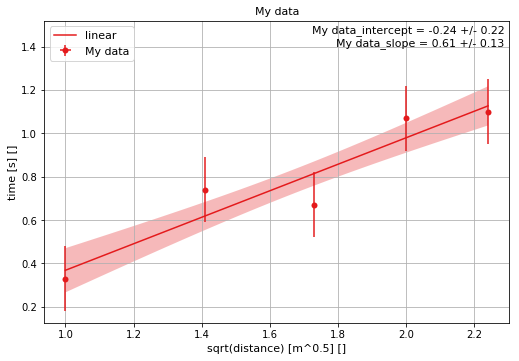
\includegraphics[width=0.75\linewidth]{files/tvssqx-1a7c2fcaca59bc03d2d4e404d143d11a.png}
\caption[]{Graph of $t$ versus $\sqrt{x}$ and line of best fit with error band.}
\label{fig:modelandexperiment:tvssqx}
\end{figure}

When plotting data and fitting them to a straight line (or other function), it is important to make sure that the experimental values have at least an uncertainty in the quantity that is being plotted on the $y$ axis. In this case, we have assumed that all of the measurements of time have an uncertainty of $0.15 {\rm s}$ and that the measurements of the distance have no (or negligible) uncertainties.

Since we expect the slope of the data to be $k$, finding the line of best fit provides us a with method to determine $k$ by using all of the data points. In this case, we find that $k=0.61\pm 0.13 {\rm s.m^{ -\frac{1}{2}}}$. \textbf{Performing a linear fit of the data is the best way to determine a constant of proportionality between the measurements}. Note that we expect the intercept to be equal to zero according to our model, but the best fit line has an intercept of $-0.24\pm 0.22 {\rm s}$, which is slightly below, but consistent, with zero. From these data, we would conclude that our measurements are consistent with Chloe's Theory. Again, remember that we can never confirm a theory, we can only exclude it; in this case, we cannot exclude Chloe's Theory with these data. If all of the data points did not sit along a straight line, we would conclude that either Chloe's Theory is invalidated, or that some form of error in the data was not taken into account.

\paragraph{Reporting measured values}

Now that you know how to attribute an uncertainty to a measured quantity and then propagate that uncertainty to a derived quantity, you are ready to present your measurement to the world. In order to conduct ``good science'', your measurements should be reproducible, clearly presented, and precisely described. Here are general rules to follow when reporting a measured number:

\begin{enumerate}
\item Indicate the units, preferably SI units (use derived SI units, such as newtons, when appropriate).
\item Include a description of how the uncertainty was determined (if it is a direct measurement, how did you choose the uncertainty? If it is a derived quantity, how did you propagate the uncertainty?).
\item Show no more than 2 ``significant digits''\footnote{Significant digits are those excluding leading and trailing zeroes.} in the uncertainty and format the central value to the same decimal as the uncertainty.
\item Use scientific notation when appropriate (usually numbers bigger than 1000 or smaller than 0.01).
\item Factor out the power 10 from the central value and uncertainty (e.g. $10123\pm 310 {\rm m}$ would be better presented as $10.12\pm 0.31 \times 10^3 {\rm m}$ or $101.2\pm 3.1 \times 10^2 {\rm m}$).
\end{enumerate}

\begin{framed}
\textbf{Checkpoint}\\
Someone has measured the average height of tables in the laboratory to be $1.0535 {\rm m}$ with a standard deviation of $0.0525 {\rm m}$. What is the best way to present this measurement?

\begin{enumerate}
\item $1.0535\pm 0.0525 {\rm m}$
\item $1.054\pm 0.053 {\rm m}$
\item $105.4\pm 5.3e -2 {\rm m}$
\item $105.35\pm 5.25 {\rm cm}$
\end{enumerate}

\begin{framed}
\textbf{Answer}\\
\begin{enumerate}[resume]
\item
\end{enumerate}
\end{framed}
\end{framed}

\paragraph{Comparing model and measurement - discussing a result}

In order to advance science, we make measurements and compare them to a theory or model prediction. We thus need a precise and consistent way to compare measurements with each other and with predictions. Suppose that we have measured a value for Chloe's constant $k= 0.44 \pm 0.09 {\rm s.m^{ -\frac{1}{2}}}$. Of course, Chloe's theory does not predict a value for $k$, only that fall time is proportional to the square root of the distance fallen. Isaac Newton's Universal Theory of Gravity does predict a value for $k$ of \$0.45 \{{\textbackslash}rm s.m\^\{-{\textbackslash}frac\{1\}\{2\}\}\} with negligible uncertainty. In this case, since the model (theoretical) value easily falls within the range given by our uncertainty, we would say that our measurement is consistent (or compatible) with the theoretical prediction.

Suppose that, instead, we had measured $k=0.55 \pm 0.08 {\rm s.m^{ -\frac{1}{2}}}$ so that the lowest value compatible with our measurement, $k=0.55 {\rm s.m^{ -\frac{1}{2}}} -0.08 {\rm s.m^{ -\frac{1}{2}}}= 0.47 {\rm s.m^{ -\frac{1}{2}}}$, is not compatible with Newton's prediction. Would we conclude that our measurement invalidates Newton's theory? The answer is: it depends... What ``it depends on'' should always be discussed any time that you present a measurement (even if your measurement \textit{is} compatible with a prediction - maybe that was a fluke). Below, we list a few common points that should be addressed when presenting a measurement that will guide you into deciding whether your measurement is consistent with a prediction:

\begin{itemize}
\item How was the uncertainty determined and/or propagated? Was this reasonable?
\item Are there systematic effects that were not taken into account when determining the uncertainty? (e.g. reaction time, parallax, something difficult to reproduce).
\item Are the relative uncertainties reasonable based on the precision that you would reasonably expect?
\item What assumptions were made in calculating your measured value?
\item What assumptions were made in determining the model prediction?
\end{itemize}

In the above, our value of $k= 0.55 \pm 0.08 {\rm s.m^{ -\frac{1}{2}}}$ is the result of propagating the uncertainty in $t$. It is thus conceivable that the true value of $t$, and therefore of $k$, is outside the range that we determined. Since our value of $k$ is still quite close to the predicted value, we would not claim to have invalidated Newton's theory with this measurement. The difference between our measurement and the predicted value is only 1.25 times $\sigma_k$, so very close to the value of the uncertainty.

In a similar way, we can discuss whether two different measurements, each with an uncertainty, are compatible with each other. If the ranges given by uncertainties in two values overlap, then they are clearly compatible. If, on the other hand, the ranges do not overlap, they could be inconsistent or the discrepancy might instead be the result of how the uncertainties were determined and the measurements could still be considered consistent with each other.

\subsubsection{Summary}

Measurable quantities have dimensions and units. A physical quantity should always be reported with units, preferably SI units.

When you build a model to predict a physical quantity, you should always ask if the prediction makes sense (Does it have a reasonable order of magnitude? Does it have the right dimensions?).

Any quantity that you measure will have an uncertainty. Almost any quantity that you determine from a model or theory will also have an uncertainty.

The best way to determine an uncertainty is to repeat the measurement and use the mean and standard deviation of the measurements as the central value and uncertainty.
If we have $N$ measurements of some quantity $t$, $\{t_1, t_2, t_3, \dots t_N\}$, then the mean, $\bar t$, and standard deviation, $\sigma_t$, are defined as:
\begin{equation}
\bar t &= \frac{1}{N}\sum_{i=1}^{i=N} t_i=\frac{t_1 +t_2 +t_3 +\dots+ t_N}{N} \\
\sigma_t^2 &=\frac{1}{N-1}\sum_{i=1}^{i=N}(t_i-\bar t)^2 = \frac{(t_1-\bar t)^2+(t_2-\bar t)^2+(t_3-\bar t)^2+\dots+(t_N-\bar t)^2}{N-1} \\
\sigma_t &=\sqrt{\sigma_t^2}
\end{equation}

You have to pay special attention to systematic uncertainties, which are difficult to determine. You should always think of ways that your measured values could be wrong, even after repeated measurements. Relative uncertainties tell you whether your measurement is precise.

There are multiple ways to propagate uncertainties. You can estimate the uncertainty using relative uncertainties or use the Min-Max method, which tends to overestimate the uncertainties. The preferred way to propagate uncertainties is with the derivative method, which you can use so long as the relative uncertainties on the measurements are small. If we have a function, $F(x,y)$ that depends on multiple variables with uncertainties (e.g. $x\pm\sigma_x$, $y\pm\sigma_y$), then the central value and uncertainty in $F(x,y)$ are given by:
\begin{equation}
\bar F &= F(\bar x, \bar y) \nonumber \\
\sigma_F &= \sqrt{\left(\frac{dF}{dx}\sigma_x \right)^2 + \left(\frac{dF}{dy}\sigma_y \right)^2 }
\end{equation}
This can be easily calculated using a computer.

If you expect two measured quantities to be linearly related (one is proportional to the other), plot them to find out! Use a computer to do so!

\begin{framed}
\textbf{Important Equations}\\
\textbf{Central value and uncertainty:}
\begin{equation}
\bar t &= \frac{1}{N}\sum_{i=1}^{i=N} t_i=\frac{t_1 +t_2 +t_3 +\dots+ t_N}{N} \\
\sigma_t^2 &=\frac{1}{N-1}\sum_{i=1}^{i=N}(t_i-\bar t)^2 = \frac{(t_1-\bar t)^2+(t_2-\bar t)^2+(t_3-\bar t)^2+\dots+(t_N-\bar t)^2}{N-1} \\
\sigma_t &=\sqrt{\sigma_t^2}
\end{equation}
\textbf{Derivative method:}
\begin{equation}
\bar F &= F(\bar x, \bar y) \nonumber \\
\sigma_F &= \sqrt{\left(\frac{dF}{dx}\sigma_x \right)^2 + \left(\frac{dF}{dy}\sigma_y \right)^2 }
\end{equation}
\begin{table}
\centering
\caption[]{How to propagate uncertainties from measured values $x\pm\sigma_x$ and $y\pm\sigma_y$ to a quantity $z(x,y)$ for common operations.}
\label{tab:modelandexperiment:prop_uncertainties}
\begin{tabular}{p{\dimexpr 0.500\linewidth-2\tabcolsep}p{\dimexpr 0.500\linewidth-2\tabcolsep}}
\toprule
\textbf{Operation to get $z$} & \textbf{Uncertainty in $z$} \\
\hline
$z=x+y$ (addition) & $\sigma_z=\sqrt{\sigma_x^2+\sigma_y^2}$ \\
$z=x -y$ (subtraction) & $\sigma_z=\sqrt{\sigma_x^2+\sigma_y^2}$ \\
$z=xy$ (multiplication) & $\sigma_z=xy\sqrt{\left(\frac{\sigma_x}{x}\right)^2+\left(\frac{\sigma_y}{y}\right)^2}$ \\
$z=\frac{x}{y}$ (division) & $\sigma_z=\frac{x}{y}\sqrt{\left(\frac{\sigma_x}{x}\right)^2+\left(\frac{\sigma_y}{y}\right)^2}$ \\
$z=f(x)$ (a function of 1 variable) & \${\textbackslash}sigma\_z={\textbackslash}left \\
\bottomrule
\end{tabular}
\end{table}
\end{framed}

\subsubsection{Thinking about the material}

\begin{framed}
\textbf{Reflect and research}\\
\begin{itemize}
\item Often, physicists will report a measured number with a ``standard'' uncertainty and indicate that there is a 68\% that the true value lies within the range covered by the uncertainty. Where does the number 68\% come from?
\item Why can the derivative method only be used when the relative uncertainties are small?
\item How would you estimate the height of a tall building?
\end{itemize}
\end{framed}

\begin{framed}
\textbf{Experiments to try at home}\\
\begin{itemize}
\item Estimate the volume of your room, and how many people could be piled into the room. State your assumptions and how you determined the values.
\end{itemize}
\end{framed}

\begin{framed}
\textbf{Experiments to try in the lab}\\
\begin{itemize}
\item Newton's Universal Theory of gravity predicts that the distance, $x$, covered by an object that has fallen for a length of time, $t$, is given by:
\end{itemize}
\begin{equation}
x = \frac{1}{2}gt^2
\end{equation}
Determine the value of $g$ (with uncertainty) by performing an experiment that will allow you to determine $g$ by determining the slope of a line of best fit.
\end{framed}

\subsubsection{Sample problems and solutions}

\paragraph{Problems}

\begin{framed}
\textbf{Problem 2.1}\\
During a physics lecture, you look under your seat and find a sheet containing data from an experiment on throwing balls vertically (perhaps a juggling experiment). The following equation is shown at the bottom of the sheet:
\begin{equation}
=\frac{v_2^{2}-v_1^{2}}{2a}
\end{equation}
along with the following description:

\begin{itemize}
\item $v_1$ = initial measured velocity of the ball ${\rm m/s}$ - various measurements.
\item $v_2$ = final measured velocity of the ball ${\rm m/s}$ - seems to be zero every time.
\item $a$ = acceleration of the ball ($-9.8 {\rm m/s^2}$).
\end{itemize}

Unfortunately, the students spilled ketchup on the left hand side of their equation, making it illegible. Luckily, you are proficient in dimensional analysis. What were the students trying to calculate, based on this model?\}
\end{framed}

\begin{framed}
\textbf{Problem 2.2}\\
Chelsea is preparing meticulously for her upcoming trip to Europe. Being a self-proclaimed ``shop-a-holic'' and physics lover, she wants to figure out how many pairs of shoes she can buy on vacation that will physically fit in her closet. Her closet is a walk-in closet with two entrance doors. Estimate the number of pairs of shoes that can fit in Chelsea's closet.
\end{framed}

\paragraph{Solutions}

\begin{framed}
\textbf{Solution 2.1}\\
We can use their equation to determine the dimension of the quantity on the left hand side:
\begin{equation}
[?]&=\frac{[v_2^{2}]-[v_1^{2}]}{[a]}=\frac{\left(\frac{L}{T}\right)^{2}-\left(\frac{L}{T}\right)^2}{\frac{L}{T^{2}}}= L
\end{equation}
Thus, the dimension of the unknown quantity is length. Given the context, they were likely attempting to model the height at which a vertically thrown ball would travel before stopping.
\end{framed}

\begin{framed}
\textbf{Solution 2.2}\\
We start by estimating the volume of Chelsea's closet as well as that of a pair of shoes. Chelsea's closet is a ``walk-in closet' with two double doors. If we know the dimensions of the door, we can estimate the width and height of the closet. Estimating the average size of a large door to be $1 {\rm m}\times 2 {\rm m}$, one face of the close will have an area of $4 {\rm m^2}$. If we estimate the depth of Chelsea's closet to be about $3 {\rm m}$, the volume of her closet is $12 {\rm m^3}$

\begin{figure}[!htbp]
\centering
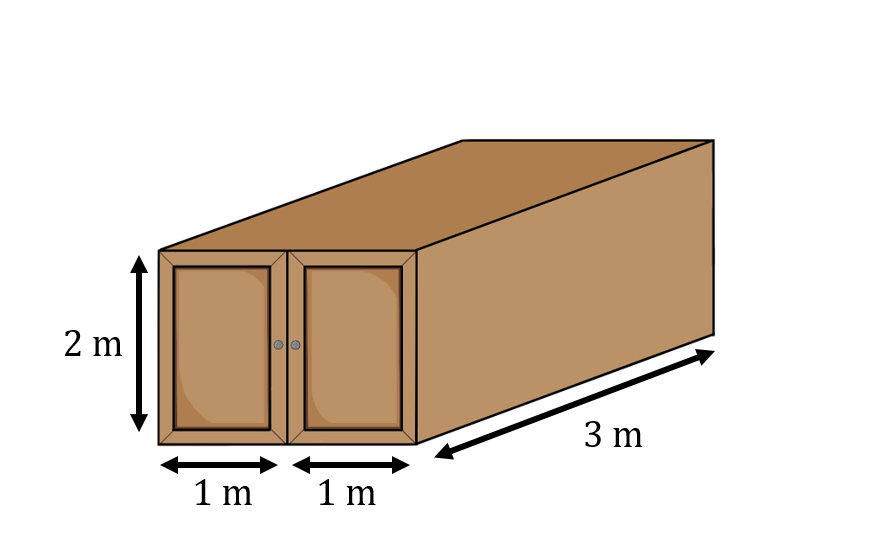
\includegraphics[width=0.4\linewidth]{files/chelseashoes-1cdd94359cfb5edcf50c4a2dafb2b741.png}
\caption[]{Chelsea's closet.}
\label{fig:modelandexperiment:chelseashoes}
\end{figure}

Next, we can estimate the size of an average pair of shoes, by modelling a shoe as a rectangular box. A single shoe has a height and width of about $5 {\rm cm}$ and a length of about $25 {\rm cm}$. A pair of shoes will thus be equivalent to box with dimensions $5 {\rm cm} \times 10 {\rm cm} \times 25 {\rm cm} = 1250 {\rm cm^3}$. This is equivalent to $0.00125 {\rm m^3}$. We can now determine how many pairs of shoes, $N$, would fit in the closet:

\begin{equation}
N=\frac{(12 {\rm m^3})}{(0.00125 {\rm m^3})}= 9600\approx 10,000
\end{equation}
We find that Chelsea can buy about 10,000 new pairs of shoes on her trip, and still fit them all into her closet. Time to get shopping, Chelsea!
\end{framed}